\chapter{Étude des déformations} \label{chap:Ch03}
\section{Grandes déformations} \label{sec:Ch03-1}
\subsection{Description de la déformation} \label{ssec:Ch03-1.1}
% Generated with LaTeXDraw 2.0.5
% Sun Nov 08 14:17:03 EST 2009
\scalebox{1} % Change this value to rescale the drawing.
{
\begin{pspicture}(0,-4)(14.744687,3.2425)
\psdots[fillstyle=solid,dotstyle=o](12.864688,1.5225)
\rput(4.8,0.7275){$\vec{\ud a}$}
\psdots[fillstyle=solid,dotstyle=o](5.0446873,0.3225)
\psdots[fillstyle=solid,dotstyle=o](5.4446874,1.3225)
\psline{->}(2.4646876,-1.2775)(2.4646876,2.3225)
\psline{->}(2.4646876,-1.2575)(6.8646874,-1.2575)
\psline{->}(2.4646876,-1.2575)(1.1046875,-2.8575)
\psbezier[linewidth=0.04](4.4646873,1.9225)(3.5646906,1.4866039)(3.1716466,0.11810785)(3.5246875,-0.8175)(3.8777285,-1.7531079)(4.424077,-2.4369879)(5.3646874,-2.0975)(6.305298,-1.7580122)(7.0475364,0.19629975)(6.6246877,1.1025)(6.2018385,2.0087004)(5.3646846,2.3583963)(4.4646873,1.9225)
\psline{->}(5.0646877,0.3225)(5.4446874,1.3425)
\psbezier[linewidth=0.02](5.0846877,0.3425)(6.0046873,1.2352536)(9.8046875,1.8425)(11.644688,0.9425)
\psdots[fillstyle=solid,dotstyle=o](11.644688,0.9225)
\psline{->}(11.684688,0.9425)(12.884687,1.5225)
\rput(6.909219,-1.5325){$x_1$}
\rput(3.1492188,2.4075){$x_2$}
\rput(1.8292187,-3.0325){$x_3$}
\rput(0.978125,0.1875){Repère fixe}
\rput(4.8392186,-0.0325){$M$}
\rput(4.8992186,1.5475){$M'$}
\rput(11.459219,0.5475){$M_t$}
\rput(13.119219,1.8475){$M_t'$}
\psbezier[linewidth=0.04](9.704687,-1.4775)(8.544687,0.0425)(11.924687,3.2225)(13.324688,2.4025)(14.724688,1.5825)(13.884687,1.1825)(12.964687,0.8225)(12.044687,0.4625)(10.864688,-2.9975)(9.704687,-1.4775)
\rput(4.845625,-2.6325){Configuration de référence}
\rput(10.955625,-2.6325){Configuration actuelle}
\rput(12.357187,-1.5125){instant $t$}
\psbezier[linewidth=0.02](5.4846873,1.3225)(7.2846875,2.4825)(10.884687,2.6425)(12.844687,1.5225)
\end{pspicture} 
}

Pour repérer la position d'une particule d'un milieu continu, il faut introduire un repère d'espace supposé fixe au cours du temps: un référentiel.
En général on choisit un référentiel galiléen, sinon il faut rajouter les forces d'inertie dans les forces de volume $f_i$.
Le mouvement est décrit par la fonction
\begin{equation}
    x_i = x_i \left( a_1, a_2, a_3, t \right) \quad i = 1, 2, 3
    \label{eq:Ch03-001}
\end{equation}
donnant la position à l'instant $t$, $M_t$, de la particule $M$ qui, dans la configuration de référence, occupe la position $\left( a_1, a_2, a_3 \right)$.
Les $x_i$ sont les variables eulériennes ou spatiales, les $a_i$ sont les variables lagrangiennes ou matérielles. 

Un vecteur matériel $\vec{\ud a} = \vec{MM'}$ devient après déformation $\vec{\ud x} = \vec{M_t M_t'}$
\begin{equation}
    \vec{\ud x_i} = \frac{\partial x_i}{\partial a_j} \ud a_j, \quad \vec{\ud x} = \mathbb{F} \vec{\ud a}
    \label{eq:Ch03-002}
\end{equation}
L'application linéaire tangente $\mathbb{F}$ qui à un vecteur matériel $\vec{\ud a}$ associe son déformation $\vec{\ud x}$ est appelée ``tenseur gradient de la déformation''.
Elle  caractérise la déformation ``locale'',  c'est-à-dire la déformation au  voisinage du point M.
Ce n'est pas cependant un mesure satisfaisante de la ``déformation'' au sens naïf du terme, car si le milieu a un mouvement de solide rigide, alors
\begin{equation}
    x_i = c_i (t) + Q_{ij} (t) a_j
    \label{eq:Ch03-003}
\end{equation}
où la matrice $Q_{ij}$ décrit une rotation et est donc orthogonale.
Le tenseur gradient de la déformation est alors donné par
\begin{equation}
    F_{ij} (a,t) = Q_{ij} (t)
    \label{eq:Ch03-004}
\end{equation}
alors qu'il n'y a manifestement pas de déformation au sens naïf du terme (variation de longueur ou variation d'angle).
En fait, le tenseur gradient de la déformation contient à la fois une rotation et une déformation.
Il convient de séparer ces deux composantes.
Par ``déformation'' on entend variation de forme, donc de longueur ou d'angle, donc encore variation de produits scalaires.
Soit $\vec{\ud a}$ et $\vec{\delta a}$ deux vecteurs matériels, $\vec{\ud x}$ et $\vec{\delta x}$ leurs déformés
\begin{equation}
    \vec{\ud x} \cdot \vec{\delta x} = \ud x_i \delta x_i = F_{ij} F_{ik} \ud a_j \delta a_k = C_{jk} \ud a_j \delta a_k
    \label{eq:Ch03-005}
\end{equation}
Ainsi la variation du produit scalaire de deux vecteurs est caractérisée par la forme bilinéaire symétrique (définie par
\begin{equation}
    C_{jk} = F_{ij} F_{ik}, \quad \mathbb{C} = \mathbb{F}^T \mathbb{F}
    \label{eq:Ch03-006}
\end{equation}
\begin{equation}
    \vec{\ud x} \cdot \vec{\delta x} = \mathbb{C} \left( \vec{\ud a}, \vec{\delta a} \right) = \vec{\ud a} \cdot \mathbb{C} \vec{\delta a}
    \label{eq:Ch03-007}
\end{equation}
$\mathbb{C}$ est le tenseur des dilatations ou tenseur de Cauchy-Green droit.
Ce tenseur est la base de la description des grandes déformations.
\begin{equation}
    \left\{
    \begin{aligned}
        & D_{ij} = F_{ik} F_{jl} \dot{C}_{kl} \\
        & \frac{\ud}{\ud t} \left( \vec{\ud x} \cdot \vec{\delta x} \right) = D_{ij} \ud x_i \partial x_j = \dot{C}_{kl} \ud a_k \ud a_l
    \end{aligned}
    \right.
    \label{eq:Ch03-008}
\end{equation}
\subsection{Le tenseur des déformations} \label{ssec:Ch03-1.2}
En l'absence de déformation, c'est à dire dans un mouvement de solide rigide \eqref{eq:Ch03-003}, on a
\begin{equation}
    C_{jk} = Q_{ij} Q_{ik} = \delta_{jk}
    \label{eq:Ch03-009}
\end{equation}
puisque la matrice $Q_{ij}$ est orthogonale.
Le tenseur des dilatations est le lenseur unité $\mathbb{1}$, et l'on a conservation du produit scalaire.
Le tenseur des déformations -- plus précisément le ``tenseur de Green-Lagrange des déformations'' -- est défini par
\begin{equation}
    \mathbb{E} = \frac{1}{2} \left( \mathbb{C} - \mathbb{1} \right), \quad E_{ij} = \frac{1}{2} \left( C_{ij} - \delta_{ij} \right)
    \label{eq:Ch03-010}
\end{equation}
Il donne la variation du produit scalaire de deux vecteurs par
\begin{equation}
    \vec{\ud x} \cdot \vec{\delta x} - \vec{\ud a} \cdot \vec{\delta a} = 2 \vec{\ud a} \cdot \mathbb{E} \vec{\delta a}
    \label{eq:Ch03-011}
\end{equation}
Comme pour le tenseur des contraintes, on démontre (voir Annexe~\ref{Ann:A}) que  dans  un  changment de repère, les composantes de  ce tenseur se transforment par
\begin{equation}
    E_{ij}' = Q_{ik} Q_{jl} E_{kl}
    \label{eq:Ch03-012}
\end{equation}
II reste à relier ce tenseur des déformations au concept physique de déformation, c'est à dire aux variations de longueur et d'angle.
\begin{defn}
    On appelle ``allongement dans la direction $\vec{n}$'', $\varepsilon \left( \vec{n} \right)$, le rapport
    \begin{equation}
        \varepsilon \vec{n} = \frac{M_tM_t' -MM}{MM'} \quad \vec{MM'} = \ud a \vec{n}
        \label{eq:Ch03-013}
    \end{equation}
    de la variation de longueur d'un vecteur matériel $MM'$ dirigé selon $\vec{n}$ de longueur initiale.
    On appelle ``glissement dans deux directions perpendiculaires $\vec{m}$ et $\vec{n}$'', la variation
    \begin{equation}
        \left( \vec{m}, \vec{n} \right) = \frac{\pi}{2} - \left( \vec{M_t M_t'}, \vec{M_tM_t''} \right) 
        \quad \left\{
        \begin{array}{l}
            \vec{MM'} = \ud a \vec{m} \\
            \vec{MM''} = \delta a \vec{n}
        \end{array}
        \right.
        \label{eq:Ch03-014}
    \end{equation}
    de l'angle de deux vecteurs matériels et $\vec{MM'}$ et $\vec{MM''}$ port\'es par $\vec{m}$ et $\vec{n}$ respectivement.
\end{defn}
\begin{thm}
    L'allongement dans une direction $\vec{n}$ et le glissement dans deux directions perpendiculaires $\vec{m}$ et $\vec{n}$ sont donnés à partir du tenseur des déformations par
    \begin{align}
        \varepsilon \left( \vec{n} \right) &= \sqrt{1 + 2 E_{ij} n_i n_j} - 1 \label{eq:Ch03-015} \\
        \gamma \left( \vec{n}, \vec{m} \right) &= \arcsin \frac{2E_{ij} m_i n_j}{\left( 1 + \varepsilon \left( \vec{m} \right) \right) \left( 1 + \varepsilon \left( \vec{n} \right) \right)} \label{eq:Ch03-016}
    \end{align}
\end{thm}
\begin{proof}
    \begin{displaymath}
        \left\{
        \begin{array}{lll}
            \vec{MM'} &= \vec{\ud a} &= \ud a \vec{n} \\
            \vec{MM''} &= \vec{\delta a} &= \delta a \vec{m}
        \end{array}
        \right.
    \end{displaymath}
    \scalebox{1} % Change this value to rescale the drawing.
    {
    \begin{pspicture}(0,-1.7917844)(10.749063,1.8396447)
    \rput(1.77,-0.6431532){\rput{27.784576}(0.38325852,-0.21540357){\psaxes[linewidth=0.02,labels=none,ticks=none,ticksize=0.10583333cm]{->}(0,0)(0,0)(2,2)}}
    \rput(2.060721,-0.8185807){\rput{27.784576}(0.09253753,-0.039976083){\psaxes[linewidth=0.06,labels=none,ticks=none,ticksize=0.10583333cm]{->}(0,0)(0,0)(1,1)}}
    \psline[linewidth=0.02cm,arrowsize=0.05291667cm 2.0,arrowlength=1.4,arrowinset=0.4]{->}(3.57,-0.8431532)(7.57,-0.8431532)
    \rput(5.5346875,-0.5381532){Déformation}
    \psline[linewidth=0.06cm,arrowsize=0.05291667cm 2.0,arrowlength=1.4,arrowinset=0.4]{->}(8.37,-0.8431532)(9.77,-0.8431532)
    \psline[linewidth=0.06cm,arrowsize=0.05291667cm 2.0,arrowlength=1.4,arrowinset=0.4]{->}(8.37,-0.8431532)(9.17,0.3568468)
    \psline[linewidth=0.06cm,linestyle=dashed,dash=0.16cm 0.16cm](8.37,-0.8431532)(8.37,0.5568468)
    \psarc[linewidth=0.04](8.37,-0.8431532){1.0}{56.309933}{90.0}
    \rput(8.284532,-1.1381532){$M_t$}
    \rput(10.124531,-1.1381532){$M_t'$}
    \rput(9.564531,0.4618468){$M_t''$}
    \rput(8.694531,0.4618468){$\alpha$}
    \rput(2.3245313,-1.1381532){$M$}
    \rput(2.9645312,-0.1381532){$M'$}
    \rput(1.2045312,-0.1381532){$M''$}
    \rput(4.0645313,-0.1381532){$\vec{n}$}
    \rput(0.9245312,0.8618468){$\vec{m}$}
    \end{pspicture} 
    }

    \begin{displaymath}
        \left\{
        \begin{array}{ll}
            \vec{M_t M_t'} &= \vec{\ud x} \\
            \vec{M_t M_t''} &= \vec{\delta x}
        \end{array}
        \right.
    \end{displaymath}
    Par définition de $\varepsilon \left( \vec{n} \right)$ et d'après \eqref{eq:Ch03-011}, on a
    \begin{displaymath}
        \varepsilon \left( \vec{n} \right) = \frac{M_t M_t' - MM'}{MM'} = \frac{|\vec{\ud x}| - \vec{\ud a}}{\ud a}
    \end{displaymath}
    \begin{eqnarray*}
        |\vec{\ud x}| &= \sqrt{\vec{\ud x} \cdot \vec{\ud x}} = \sqrt{\vec{\ud a}\cdot\vec{\ud a} + 2 \vec{\ud a}\cdot \mathbb{E} \ud a} \\
        &= \ud a \sqrt{\vec{n}\cdot\vec{n} + 2\vec{n}\cdot\mathbb{E}\vec{n}} = \ud a \sqrt{1 + 2 \vec{n}\cdot \mathbb{E} \vec{n}}
    \end{eqnarray*}
    et on obtient directement \eqref{eq:Ch03-015}.
    De même, on peut écrire à partir de \eqref{eq:Ch03-014}
    \begin{eqnarray*}
        \sin \gamma \left( \vec{m},\vec{n} \right) &= \cos \left( \vec{M_tM_t'}, \vec{M_tM_t''} \right) \\
        &= \frac{\vec{M_tM_t'}\cdot \vec{M_tM_t''}}{M_t M_t'\ M_t M_t''} = \frac{\vec{\ud x}\vec{\delta x}}{|\vec{\ud x}||\vec{\delta x}|}
    \end{eqnarray*}
    mais d'après \eqref{eq:Ch03-011} et \eqref{eq:Ch03-013}
    \begin{displaymath}
        |\vec{\ud x}| = \ud a \left( 1 + \varepsilon \left( \vec{n} \right) \right)
    \end{displaymath}
    \begin{displaymath}
        \vec{\ud x} \cdot \vec{\delta x} = \vec{\ud a} \cdot \vec{\delta a} + 2 \vec{\ud a}\cdot \mathbb{E} \vec{\delta a} = 2 \ud a \delta a \vec{m} \cdot \mathbb{E} \vec{n}
    \end{displaymath} 
    puisque $\vec{m}$ est perpendiculaire à $\vec{n}$.
    Finalement
    \begin{displaymath}
        \sin \gamma \left( \vec{m}, \vec{n} \right) = \frac{2\vec{m}\cdot \mathbb{E} \vec{n}}{\left( 1 + \varepsilon \left( \vec{n} \right) \right)\left( 1 + \varepsilon \left( \vec{m} \right) \right)}
    \end{displaymath}
    ce qui donne \eqref{eq:Ch03-016}.
\end{proof}

En particulier, on obtient la signification des composantes de $C_{ij}$ de $\mathbb{C}$ en appliquant \eqref{eq:Ch03-015} et \eqref{eq:Ch03-016} aux vecteurs de base
\begin{eqnarray}
    E_{11} &= \vec{e}_1 \cdot \mathbb{E} \vec{e}_1 &= \frac{1}{2} \left\{ \left[ 1 + \varepsilon \left( \vec{e}_1 \right) \right]^{2} -1 \right\} \label{eq:Ch03-017}\\
    E_{12} &= \vec{e}_1 \cdot \mathbb{E} \vec{e}_2 &= \frac{1}{2} \left[ 1 + \varepsilon \left( \vec{e}_1 \right) \right]\left[ 1 + \varepsilon \left( \vec{e}_2 \right) \right] \sin \gamma \left( \vec{e}_1, \vec{e}_2 \right)  \label{eq:Ch03-018}
\end{eqnarray}
Ainsi les composantes diagonales de $E_{ij}$ caractérisent les allongements dans les directions des axes, tandis que les composantes non diagonales caractérisent les glissements dans les directions des axes.
On peut donc, à partir de ces composantes, construire la déformée d'un cube unité d'arête dirigée selon les axes: ce cube se déforme en parallélépipède défini par
\begin{center}
    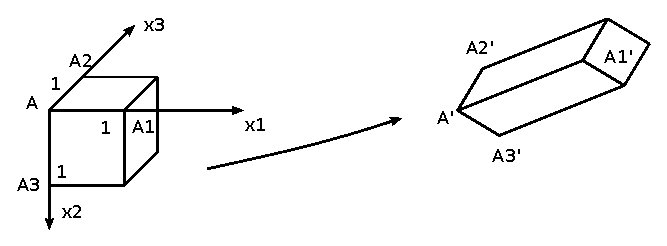
\includegraphics{../images/T1_Ch03-0003}
\end{center}
\begin{equation}
    \left\{
    \begin{aligned}
        A'A_1' &= \sqrt{1+2E_{11}}\\
        \left( A'A_1',\ A'A_2' \right) &= \arcsin \frac{2E_{12}}{\sqrt{1+2E_{11}}\sqrt{1+2E_{22}}}
    \end{aligned}
    \right.
    \label{eq:Ch03-019}
\end{equation}

Comme pour le tenseur des contraintes, on peut diagonaliser le tenseur des déformations, c'est à dire trouver un repère orthogonal où la matrice représentant $\mathbb{E}$ est diagonale, $E_1$, $E_2$ et $E_3$ sont appelés allongements
\begin{equation}
    \mathbb{E} = 
    \begin{bmatrix}
        E_1 & 0 & 0 \\
        0 & E_2 & 0 \\
        0 & 0 & E_3
    \end{bmatrix}
    \label{eq:Ch03-020}
\end{equation}
principaux.
La propriété caractéristique des axes principaux des déformations est que les glissements dans leur direction sont nuls.
Un cube unité d'arête dirieée selon les axes principaux se transforme en un parallélépipède rectange
\begin{center}
    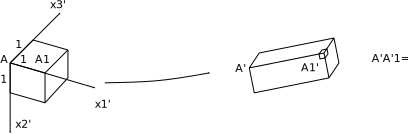
\includegraphics{../images/T1_Ch03-0004}
\end{center}

En mécanique des solides, on introduit souvent le vecteur déplacement $\vec{u} = \vec{x}-\vec{a}$, définissant le mouvement par
\begin{equation}
    x_i = a_i + u_i \left( a_1, a_2, a_3, t \right)
    \label{eq:Ch03-021}
\end{equation}
On obtient alors à partir de \eqref{eq:Ch03-022}
\begin{equation}
    F_{ij} = \delta_{ij} + \frac{\partial u_i}{\partial a_j}
    \label{eq:Ch03-022}
\end{equation}
Le tenseur des déformations est alors donné par
\begin{equation}
    E_{ij} = \frac{1}{2} \left( \frac{\partial u_i}{\partial a_j} + \frac{\partial u_j}{\partial a_i} + \frac{\partial u_k}{\partial a_i}\frac{\partial u_k}{\partial a_j} \right)
    \label{eq:Ch03-023}
\end{equation}
\section{Petites déformations} \label{sec:Ch03-2}
\subsection{Hypothèse des petites perturbations} \label{ssec:Ch03-2.1}
En Mécanique des Solides, on fait souvent l'hypothèse:
\par\noindent\textbf{Hypothèse des petites perturbations.} Le solide s'écarte peu de sa configuration de référence.

Les déplacements et les déformations restent petits. 
Ceci a deux conséquences essentielles 
\begin{enumerate}
    \item On peut identifier variables de Lagrange $a_i$ et variables d'Euler $x_i$, dans la mesure où la différence entre les deux est négligeable.
        Ceci est tout à fait essentiel, car certaines équations s'écrivent naturellement en variables eulériennes -- les équations d'équilibre par exemple -- alors que d'autres s'écrivent plus naturellement en variables lagrangiennes -- la définition des déformations par exemple.
        Entres autres, cela revient à écrire les équations d'équilibre dans la configuration telle qu'elle existe avant déformation, alors qu'il faudrait, en toute rigueur, les écrire dans la configuration réelle où s'appliquent effectivement les efforts.
        Cette approximation habituellement appelée hypothèse de linéarité externe, est habituellement justifiée, mais on rencontrera quelques cas, en particulier toutes les questions de stabilité, où elle ne l'est pas.
    \item Dans tous les calculs,, on ne conserve que les termes les plus significatifs, en négligeant les termes d'ordre supérieur en $u_i$ et ses dérivées.
        En d'autres termes, on effectue une linéarisation autour de la configuration de référence, supposée naturelle, c'est à dire libre de contraintes, cararctérisée par 
        \begin{equation}
            \rho = \rho_c, \quad u_i = 0, \quad \sigma_{ij} = 0
            \label{eq:Ch03-024}
        \end{equation}
        et le mouvement est décrit par
        \begin{equation}
            \rho = \rho_0 + \rho, \quad u_i, \quad \sigma_{ij}
            \label{eq:Ch03-025}
        \end{equation}
        avec $\rho'$, $u_i$, $\sigma_{ij}$ petits et fonctions de $\left( x_i,t \right)$, $x_i$ représentant indifféremment les variables de Lagrange $a_i$ ou d'Euler $x_i$.
        La vitesse $V_i$ et l'accélération $\gamma_i$ sont données par
        \begin{equation}
            V_i = \frac{\partial u_i}{\partial t}, \quad \gamma_i = \frac{\partial^2 u_i}{\partial t^2}
            \label{eq:Ch03-026}
        \end{equation}
        en remarquant que les dérivées particulaires sont des dérivées partielles par rapport au temps en variables de Lagrange.
        L'équation de continuité~\eqref{eq:Ch01-011} donne
        \begin{equation*}
            \frac{\ud}{\ud t} \left( \rho_0 +\rho' \right) + \left( \rho_0 + \rho' \right) \frac{\partial V_i}{\partial x_i} = 0
        \end{equation*}
        mais  $\ud \rho_0 / \ud t$, $\ud \rho' / \ud t = \partial \rho' / \partial t$ en variables de Lagrange, et on peut négliger le  terme $\rho' \partial V_i / \partial x_i$ qui est du second ordre par rapport à la perturbation.
        Il  reste  donc
        \begin{equation*}
            \frac{\partial \rho'}{\partial t} + \rho_0' \frac{\partial^2 u_i}{\partial x_i \partial t} = 0
        \end{equation*}
        ou en intégrant par rapport au temps
        \begin{equation}
            \rho' = - \rho_0 \frac{\partial u_i}{\partial x_i}
            \label{eq:Ch03-027}
        \end{equation}
        la constante d'intégration étant nulle puisque dans la configuration de référence $\rho'$ et $u_i$ sont nuls.
        Nous retrouverons cette relation au paragraphe~\ref{ssec:Ch03-2.2}.
        De même, 1'équation du mouvement \eqref{eq:Ch01-015} donne
        \begin{equation}
            \rho_0 \frac{\partial^2 u_i}{\partial t^2} = \frac{\partial \sigma_{ij}}{\partial x_j} + f_i
            \label{eq:Ch03-028}
        \end{equation}
\end{enumerate}
En particulier,  on constate que $\rho'$ disparaît disparaît de l'équation du mouvement.
En Mécanique des Solides, on peut oublier l'équation de continuité qui permet seulement de calculer $\rho'$ par \eqref{eq:Ch03-027} une fois connu le déplacement $u_i \left( x_i, t \right)$.
\subsection{Tenseur linéarisé des déformations} \label{ssec:Ch03-2.2}
Dans le cadre d'hypothèse des petites perturbations, le tenseur des déformations introduit au paragraphe~\ref{ssec:Ch03-1.2} et défini par \eqref{eq:Ch03-023} à partir du déplacement $u_i$ devient
\begin{equation}
    \varepsilon_{ij} = \frac{1}{2} \left( \frac{\partial u_i}{\partial x_j} + \frac{\partial u_j}{\partial x_i} \right)
    \label{eq:Ch03-029}
\end{equation}
Ce tenseur $\varepsilon_{ij}$ est le tenseur des déformations linéarisées.
En grandes déformations, en effet, le tenseur de Green-Lagrange que nous avons défini, n'est pas le seul possible, et on peut en introduire bien d'autres, mais en petites déformations, tous ces tenseurs se réduisent au tenseur $\mathbb{\varepsilon}$ défini par~\eqref{eq:Ch03-029}.
Par linéarisation des formules \eqref{eq:Ch03-015} et \eqref{eq:Ch03-016}, il permet de calculer l'allongement dans une direction $\vec{n}$ le glissement dans deux directions $\vec{m}$ et $\vec{n}$ par les formules
\begin{align}
    \varepsilon \left( \vec{n} \right) &= \varepsilon_{ij} n_i n_j \label{eq:Ch03-030} \\
    \gamma \left( \vec{m}, \vec{n} \right) &= 2 \varepsilon_{ij} n_i m_j \label{eq:Ch03-031} 
\end{align}
obtenues simplement par développement limité des diverses fonctions internenant dans \eqref{eq:Ch03-015} et \eqref{eq:Ch03-016}.
On obtient aussi la signification des composantes $\varepsilon_{ij}$
\begin{align}
    \varepsilon \left( \vec{e}_1 \right) &= \varepsilon_{11} = \frac{\partial u_1}{\partial x_1} \label{eq:Ch03-032} \\
    \gamma \left( \vec{e}_1, \vec{e}_2 \right) &= \gamma_{12} = 2 \varepsilon_{12} = \left( \frac{\partial u_1}{\partial x_2} + \frac{\partial u_2}{\partial x_1} \right) \label{eq:Ch03-033}
\end{align}
Pour dégager la signification de ce tenseur, on peut considérer le mouvement du voisinage d'un point $M$ on peut écrire
\begin{align*}
    \left( \overrightarrow{M'M_t'} \right)_i &= u_i \left( x + \ud x \right) \\
    &= u_i (x) + \frac{\partial u_i}{\partial x_j} (x) \ud x_j\\
    &= u_i + U_{i,j} \ud x_j
\end{align*}
On décompose alors $u_{i,j}$ en partie symétrique et antisymétrique
\begin{equation*}
    \left( \overrightarrow{M'M_t'} \right)_i = u_i + \omega_{ij} \ud x_j + \varepsilon_{ij} \ud x_j
\end{equation*}
\begin{equation}
    \varepsilon_{ij} = \frac{1}{2} \left( u_{i,j} + u_{j,i} \right), \quad \omega_{ij} = \frac{1}{2} \left( u_{i,j} - u_{j,i} \right)
    \label{eq:Ch03-034}
\end{equation}
On introduit le vecteur $\vec{\omega}$, adjoint du tenseur antimétrique $\omega_{ij}$ (Annexe~\ref{Ann:A}) par
\begin{equation}
    \omega_{ij} =
    \begin{bmatrix}
        0 & \omega_{12} & \omega_{13} \\
        \omega_{21} & 0 & \omega_{23} \\
        \omega_{31} & \omega_{32} & 0
    \end{bmatrix}
    =
    \begin{bmatrix}
        0 & -\omega_{3} & \omega_{2} \\
        \omega_{3} & 0 & -\omega_{1} \\
        -\omega_{2} & \omega_{1} & 0
    \end{bmatrix}
    \label{eq:Ch03-035}
\end{equation}
ce qui permet d'écrire pour $\omega_{ij} \ud x_j$
\begin{equation}
    \begin{bmatrix}
        0 & -\omega_{3} & \omega_{2} \\
        \omega_{3} & 0 & -\omega_{1} \\
        -\omega_{2} & \omega_{1} & 0
    \end{bmatrix}
    \begin{bmatrix}
        \ud x_1 \\
        \ud x_2 \\
        \ud x_3
    \end{bmatrix}
    =
    \begin{bmatrix}
        \omega_2 \ud x_3 - \omega_3 \ud x_2 \\
        \omega_3 \ud x_1 - \omega_1 \ud x_3 \\
        \omega_1 \ud x_2 - \omega_2 \ud x_1
    \end{bmatrix}
    \begin{bmatrix}
        \omega_1 \\
        \omega_2 \\
        \omega _3
    \end{bmatrix}
    \wedge 
    \begin{bmatrix}
        \ud x_1 \\
        \ud x_2 \\
        \ud x_3
    \end{bmatrix}
    \label{eq:Ch03-036}
\end{equation}
et finalement on a
\begin{equation}
    \overrightarrow{M'M_t'} = \underbrace{\underbrace{\vec{u}}_{\text{translation}} + \underbrace{\vec{\omega} \wedge \vec{\ud x}}_{\text{rotation}}}_{\text{mouvement rigidifiant}} + \underbrace{\mathbb{\varepsilon} \vec{\ud x}}_{\text{déformation pure}}
     \label{eq:Ch03-037}
\end{equation}
Le mouvement rotation et du voisinage d'un point $M$ se  compose  d'une  translation, d'une rotation et d'une déformation pure.

On peut refaire sur le tenseur des déformations tout ce que nous avons fait au chapitre~\ref{chap:Ch02} sur le tenseur des contraintes: diagonalisation, définition des invariants, décomposition en déviateur et partie sphérique
\begin{equation}
    \left\{
    \begin{aligned}
        \varepsilon_{ij} &= \mathbb{\varepsilon} \delta_{ij} + e_{ij} \\
        \varepsilon & = \frac{\varepsilon_{ii}}{3} = \frac{\varepsilon_{11} + \varepsilon_{22} + \varepsilon_{33}}{3} = \frac{\varepsilon_1 + \varepsilon_2 + \varepsilon_3}{3} \\
        e_{ij} &= \varepsilon_{ij} - \frac{1}{3} \varepsilon_{kk} \delta_{ij}, \quad e_{ii} = 0
    \end{aligned}
    \right.
    \label{eq:Ch03-038}
\end{equation}

Physiquement, cette décomposition correspond à la décomposition de la déformation en une dilatation uniforme (partie sphérique) et une distorsion, c'est à dire une déformation sans changement de volume (déviateur).
En effet, on vérifie facilement que la trace $\varepsilon_{ii}$ du tenseur des déformations est égale à la variation relative de volume
\begin{equation}
    \frac{\Delta V}{V} = \varepsilon_{ii} = 3\varepsilon
    \label{eq:Ch03-039}
\end{equation}
Il suffit par exemple de partir d'un élément de volume parallélépipédique orienté selon les directions principales du tenseur des déformations

Après déformation, cet élément devient un parallélépipède rectangle de côté $(1+\varepsilon_1)\ud x_1$, $(1+\varepsilon_2)\ud x_2$, $(1+\varepsilon_3)\ud x_3$ et son volume est
\begin{align*}
    V+\Delta V &= (1+\varepsilon_1)(1+\varepsilon_2)(1+\varepsilon_3)\ud x_1 \ud x_2 \ud x_3 \\
    &= \left[ 1 + \left( \varepsilon_1 + \varepsilon_2 + \varepsilon_3 \right) \right] V
\end{align*}
en négligeant les termes d'ordre 2 en $\varepsilon_1$, $\varepsilon_2$, $\varepsilon_3$, ce qui donne directement \eqref{eq:Ch03-039}.
La conservation de la masse
\begin{equation*}
    \left( \rho_0 + \rho' \right) \left( V + \Delta V \right) = \rho_0 V
\end{equation*}
donne alors
\begin{equation}
    \frac{\rho'}{\rho_0} = - \frac{\Delta V}{V} = - \varepsilon_{ii} = - u_{i,i}
    \label{eq:Ch03-040}
\end{equation}
et on retrouve \eqref{eq:Ch03-027}.
Nous terminons ce paragraphe par quelques exemples de déformatjons homogènes.
\begin{enumerate}
    \item Dilatation uniforme
        \begin{equation}
            \left\{
            \begin{aligned}
                u_i &= \alpha x_i \\
                \varepsilon_{ij} &= u_{i,j} = \alpha \delta_{ij}, \quad \frac{\Delta V}{V} = 3\alpha
            \end{aligned}
            \right.
            \label{eq:Ch03-041}
        \end{equation}
    \item Extension simple
        \begin{equation}
            \left\{
            \begin{aligned}
                u_1 &= \alpha x_1 \\
                u_2 &= -\beta x_2 \\
                u_3 &= -\beta x_3
            \end{aligned}
            \right. \qquad
            \mathbb{\varepsilon} = 
            \begin{bmatrix}
                \alpha & 0 & 0 \\
                0 & -\beta & 0 \\
                0 & 0 & -\beta
            \end{bmatrix}
            \label{eq:Ch03-042}
        \end{equation}
        Si cette extension se fait sans changement de volume, alors d'après \eqref{eq:Ch03-039}, on a $\beta = \frac{\alpha}{2}$.
        La décomposition en déviateur et partie sphérique s'écrit comme en \eqref{eq:Ch01-019}
        \begin{equation}
            \mathbb{\varepsilon} = \varepsilon 
            \begin{bmatrix}
                1 & 0 & 0 \\
                0 & 1 & 0 \\
                0 & 0 & 1
            \end{bmatrix}
            + e 
            \begin{bmatrix}
                1 & 0 & 0 \\
                0 & -\frac{1}{2} & 0 \\
                0 & 0 & -\frac{1}{2}
            \end{bmatrix}
            , \quad e \frac{2 \left( \alpha - \beta \right)}{3}
            \label{eq:Ch03-043}
        \end{equation}
    \item Glissement simple
        \begin{equation}
            \left\{
            \begin{aligned}
                u_1 &= \gamma x_1 \\
                u_2 &= 0 \\
                u_3 &= 0
            \end{aligned}
            \right. \qquad
            u_{i,j}' = 
            \begin{bmatrix}
                0 & \gamma & 0 \\
                0 & 0 & 0 \\
                0 & 0 & 0
            \end{bmatrix}
            \label{eq:Ch03-044}
        \end{equation}
        \begin{equation}
            \mathbb{\varepsilon} = 
            \begin{bmatrix}
                0 & \frac{\gamma}{2} & 0 \\
                \frac{\gamma}{2} & 0 & 0 \\
                0 & 0 & 0
            \end{bmatrix}, \quad
            \mathbb{\omega} = 
            \begin{bmatrix}
                0 & \frac{\gamma}{2} & 0 \\
                -\frac{\gamma}{2} & 0 & 0 \\
                0 & 0 & 0
            \end{bmatrix}, \quad
            \vec{\omega} = 
            \begin{bmatrix}
                0 \\
                0 \\
                \frac{-\gamma}{2}
            \end{bmatrix}
            \label{eq:Ch03-045}
        \end{equation}
        Le mouvement se compose de la déformation définie par $\varepsilon$ et d'une rotation de $\frac{-\gamma}{2}$ autour de l'axe $x_3$.

        Pour visualiser les déformations, on a représenté des déformations importantes, mais il ne faut pas oublier que les déformations sont en fait petites: $\alpha$, $\beta$, $\gamma$ sont des quantités petites.
\end{enumerate}
\subsection{Dualité contraintes--déformations} \label{ssec:Ch03-2.3}
On remarque l'analogie entre le tenseur des déformations $\varepsilon_{ij}$, défini par \eqref{eq:Ch03-029} à partir du déplacement $u_i$ et le tenseur des taux de déformations $D_{ij}$ défini par \eqref{eq:Ch01-023} à partir des vitesses $V_i$.
Tout ce que nous avons fait au paragraphe~\ref{ssec:Ch03-2.2} sur le petit déplacement $u_i$, en particulier toutes les interprétations physiques, peut se transposer directement aux vitesses $V_i$ qui représentent le déplacement infinitésimal entre la configuration à l'instant $t$ et celle à l'instant $t+\ud t$.
Plus précisément, on a l'analogie suivante
\begin{center}
    \begin{tabular}[c]{lccr}
        Déplacements & $u_i$ & $V_i$ & Vitesses \\
        gradient des déplacements & $u_{i,j}$ & $V_{i,j}$ & gradient des vitesses \\
        tenseur des déformations & $\varepsilon_{ij}$ & $D_{ij}$ & tenseur des taux de déformation \\
        tenseur des rotations & $\omega_{ij}$ & $\Omega_{ij}$ & tenseur taux de rotation \\
        vecteur rotation & $\vec{\omega}$ & $\vec{\Omega}$ & vecteur taux de rotation \\
        allongement dans la direction $\vec{n}$ & $\varepsilon (\vec{n})$ & & taux d'allongement \\
        glissement dans les directions $\vec{m}$, $\vec{n}$ & $\gamma (\vec{m},\vec{n})$ & & taux de glissement \\
        etc.
    \end{tabular}
\end{center}

Réciproquement, tout ce que nous avons fait au paragraphe~\ref{ssec:Ch03-1.2} peut se transposer directement en termes de déplacements.
Il s'agit simplement d'un changement de terminologie.
On parle de déplacement virtuel $\displaystyle{\mathop{u}^{*}}_i$ au lieu de vitesses virtuelles $\displaystyle{\mathop{V}^{*}}_i$ et de "travaux virtuels" au lieu de "puissances virtuelles".
Par exemple, \eqref{eq:Ch01-024} ou \eqref{eq:Ch01-038} peut s'écrire
\begin{equation}
    \iiint_{\Omega} \rho \gamma_i {\mathop{u}^*}_i \ud v = \iiint_{\Omega} f_i {\mathop{u}^*}_i \ud v + \iint_{\partial \Omega} T_i {\mathop{u}^*}_i \ud S - \iiint_{\Omega} \sigma_{ij} {\mathop{\varepsilon}^*}_{ij} \ud v
    \label{eq:Ch03-046}
\end{equation}
expression du théorème des travaux virtuels ou du principe des travaux virtuels, suivant le point de vue que l'on adopte.

En particulier, le travail des efforts intérieurs par unité de volume est
\begin{equation}
    {\mathop{w}^*}_{int} = \sigma_{ij} {\mathop{\varepsilon}^*}_{ij}
    \label{eq:Ch03-047}
\end{equation}
qui met en dualité le tenseur des contraintes $\sigma_{ij}$ que nous avons étudié au chapitre~\ref{chap:Ch02}, et le tenseur des déformations $\varepsilon_{ij}$ que nous venons d'introduire.
C'est une propriété tout à fait universelle: dans toute théorie des milieux continus, il y a dualité entre les contraintes et les déformations, c'est à dire entre la schématisation des efforts intérieurs et la description cinématique.
Dans le cadre de la MMC classique, que nous développons actuellement, cela n'apporte qu'une simple vérification.
Dans d'autres cas, où la schématisation à adopter est moins évidente, cela sera pour nous un guide précieux.

On peut pousser plus loin cette dualité, en remarquant que dans toute théorie des milieux continus, on travaille sur quatre espaces\\
\begin{tabular}{lll}
    - l'espace des déplacements &$\mathcal{U} $&$ u \in \mathcal{U}$ \\
    - l'espace des déformations &$\mathcal{D} $&$ \varepsilon \in \mathcal{D}$ \\
    - l'espace des contraintes  &$\mathcal{S} $&$ \sigma \in \mathcal{S}$ \\
    - l'espace des chargements  &$\mathcal{C} $&$ \phi = \left( f_i, T_i^e \right) \in \mathcal{C}$ \\
\end{tabular}

Le travail des efforts extérieurs met en dualité $\mathcal{U}$ et $\mathcal{C}$ par
\begin{equation}
    \langle u, \phi \rangle = \iiint_{\Omega} u_i f_i \ud v + \iint_{\partial \Omega} u_{i} T_i^e \ud S
    \label{eq:Ch03-048}
\end{equation}
Le travail des efforts intérieurs met en dualité $\mathcal{D}$ et $\mathcal{S}$ par
\begin{equation}
    \langle\langle \varepsilon, \sigma \rangle\rangle = \iiint_{\Omega} \sigma_{ij} \varepsilon_{ij} \ud v
    \label{eq:Ch03-049}
\end{equation}
et, en statique, le théorème des travaux virtuels \eqref{eq:Ch03-046} peut s'écrire
\begin{equation}
    \langle\langle \mathop{\varepsilon}^* , \sigma \rangle \rangle = \langle \mathop{u}^* , \phi \rangle
    \label{eq:Ch03-050}
\end{equation}

Nous reviendrons sur cette dualité lorsque nous parlerons des méthodes variationnelles (chapitre \ref{chap:Ch09}).
\section{Compatibilite des déformations} \label{sec:Ch03-3}
Connaissant le champ des déplacements $u_i (x)$ on en déduit par \eqref{eq:Ch03-029} le champ des déformations $\varepsilon_{ij}(x)$.
Réciproquement, si on connaît le champ des déformations $\varepsilon_{ij}(x)$, peut-on calculer le champ des déplacements $u_i (x)$ ?
Et si oui, comment?
Le premier problème est celui de la compatibilité des déformations, le second celui de l'intégration d'un champ de déplacements.
Ce problème est extrêmement important en mécanique des solides, car nous verrons que la solution s'obtient souvent sous forme d'un champ de déformation; il faut alors remonter aux déplacements.
Remarquons que, en vertu de l'analogie discutée au paragraphe~\ref{ssec:Ch03-2.3}, on pourra transposer tous nos résultats en termes de vitesse et de taux de déformation, le problème étant alors de calculer le champ des vitesses à partir de la valeur en tout point du tenseur taux de déformation.
\subsection{Calcul de la rotation} \label{ssec:Ch03-3.1}
Pour calculer le déplacement $u_i$, il faut intégrer les formes différentielles 
\begin{equation}
    \ud u_i = u_{i,j} \ud x_j = \left( \varepsilon_{ij} + \omega_{ij} \right) \ud x_j
    \label{eq:Ch03-051}
\end{equation}
Or. on connaît $\varepsilon_{ij}(x)$ mais on ne connaît pas $\omega_{ij}$.
La première étape consiste donc à calculer la rotation $\omega_{ij}$.
\begin{lem} \label{lem:Ch03-1}
    Les dérivées de la rotation sont liées à celles de la déformation par la relation
    \begin{equation}
        \omega_{ij,l} = \varepsilon_{il,j} - \varepsilon_{jl,i}
        \label{eq:Ch03-052}
    \end{equation}
\end{lem}
\begin{proof}
    On part de la définition 
    \begin{align*}
        \omega_{ij} &= \frac{1}{2} \left( u_{i,j} - u_{j,i} \right) \\
        &= \frac{1}{2} \left( u_{i,jl} - u_{j,il} \right) = \frac{1}{2} \left( u_{i,jl} + u_{l,ij} - u_{l,ij} - u_{j,il} \right) \\
        &= \frac{1}{2} \left( u_{i,l} + u_{l,i} \right)_{,j} - \frac{1}{2} \left( u_{l,j} + u_{j,l} \right)_{,i} \\
        &= \varepsilon_{il,j} - \varepsilon_{jl,i}
    \end{align*}
    en utilisant le fait que les dérivées partielles commutent: $u_{i,jl} = u_{i,lj}$, etc.
\end{proof}

On peut alors calculer la rotation $\omega_{ij}$ par intégration du système
\begin{equation}
    \ud \omega_{ij} = \left( \varepsilon_{il,j} - \varepsilon_{jl,i} \right) \ud x_l
    \label{eq:Ch03-053}
\end{equation}
\begin{lem} \label{lem:Ch03-2}
    Une CNS pour que le système 
    \begin{equation}
        \ud f = a_l \ud x_l
        \label{eq:Ch03-054}
    \end{equation}
    soit intégrable, c'est à dire pour que l'on puisse calculer $f$ à partir des $a_l = f_{,l}$ est que 
    \begin{equation}
        a_{l,m} = a_{m,l}
        \label{eq:Ch03-055}
    \end{equation}
\end{lem}
\begin{proof}
    La CN est évidente (elle exprime simplement que $f_{,lm} = f_{,ml}$).
    On démontre en mathématiques que cette condition est également suffisante.
\end{proof}

En appliquant ce lemme au système différentiel \eqref{eq:Ch03-053}, on obtient la condition suivante
\begin{equation}
    \begin{aligned}
        \left( \varepsilon_{il,j} -\varepsilon_{jl,i} \right)_{,k} = \left( \varepsilon_{ik,j} - \varepsilon_{jk,i} \right)_{,l} \\
        \varepsilon_{il,jk} + \varepsilon_{jk,il} - \varepsilon_{jl,ik} - \varepsilon_{ik,jl} = 0
    \end{aligned}
    \label{eq:Ch03-056}
\end{equation}
Cette condition est une CNS pour que l'on puisse calculer $\omega_{ij}$ à partir de $\varepsilon_{ij}$.
C'est donc une condition nécessaire pour que le champ de déformation $\varepsilon_{ij}$ soit intégrable, c'est à dire pour que l'on puisse calculer le déplacement $u_i$.

On tire également du Lemme~\ref{lem:Ch03-1} le résultat suivant
\begin{thm} \label{thm:Ch03-2}
    Si le champ de déformation est identiquement nul, alors le déplacement est un déplacement de solide rigide 
    \begin{equation}
        \vec{u} = \vec{c} + \vec{\omega} \wedge \vec{x}
        \label{eq:Ch03-057}
    \end{equation}
\end{thm}
Il est en effet clair que si le déplacement est un déplacement de solide rigide (infinitésimal, bien entendu), alors le tenseur des déformations associé est nul, puisque $u_{i,j}$ est antisymétrique.
Le théorème~\ref{thm:Ch03-2} constitue une réciproque.
Compte-tenu de l'analogie présentée au paragraphe~\ref{ssec:Ch03-2.3}, ce théorème est identique au Lemme~\ref{lem:Ch01-3} paragraphe~\ref{ssec:Ch01-2.1}.

\begin{proof}
    Puisque $\varepsilon_{ij}$ est nul, le Lemme~\ref{lem:Ch03-1} montre que $\omega_{ij,l}$ est nul, et donc que $\omega_{ij}$ est constant
    \begin{equation*}
        u_{i,j} = \not{\varepsilon_{ij}} + \omega_{ij} = \omega_{ij}^0
    \end{equation*}
    Le système~\eqref{eq:Ch03-051} s'intègre alors directement pour donner
    \begin{equation*}
        u_i = \omega_{ij}^0 x_j + c_{j}^0
    \end{equation*}
    que l'on peut écrire sous la forme \eqref{eq:Ch03-057} en introduisant le vecteur $\vec{\omega}$ adjoint du tenseur antisymétrique $\omega_{ij}^0$ (le calcul est le même que celui qui a conduit à \eqref{eq:Ch03-037}.
\end{proof}
\subsection{Calcul du déplacement} \label{ssec:Ch03-3.2}
Sous réserve que la condition~\eqref{eq:Ch03-056} soit vérifiée, l'intégration du système \eqref{eq:Ch03-053} donne $\omega_{ij}$ à une constante près $\omega_{ij}^0$.
Le déplacement $u_i$ s'obtiendra alors en intégrant le système \eqref{eq:Ch03-051}
\begin{equation*}
    \ud u_i = u_{i,j} \ud x_j = \left( \varepsilon_{ij} + \omega_{ij} \right) \ud x_j
\end{equation*}
Pour que cela soit possible, il faut et il suffit, d'après le Lemme~\ref{lem:Ch03-2}, que
\begin{equation*}
    \varepsilon_{ij,l} + \omega_{ij,l} = \varepsilon_{il,j} + \omega_{il,j}
\end{equation*}
Mais les dérivées $\omega_{ij,l}$ ont été calculées par \eqref{eq:Ch03-052}, et cette condition devient 
\begin{equation*}
    \varepsilon_{ij,l} + \varepsilon_{il,j} - \varepsilon_{jl,i} = \varepsilon_{il,j} + \varepsilon_{ij,l} - \varepsilon_{jl,i}
\end{equation*}
condition qui se trouve identiquement vérifiée, et le système \eqref{eq:Ch03-051} peut toujours s'intégrer à un déplacement de la forme 
\begin{equation*}
    \omega_{ij}^0 x_j + c_i^0
\end{equation*}
près, c'est à dire à un déplacement de solide rigide près.
Nous avons donc démontré le résultat suivant
\begin{thm} \label{thm:Ch03-3}
    Pour que le champ de déformation $\varepsilon_{ij}(x)$ soit intégrable, il faut et il suffit que les ``équations de compacibilité'' \eqref{eq:Ch03-056}
    \begin{equation*}
        \varepsilon_{il,jk} + \varepsilon_{jk,il} - \varepsilon_{jl,ik} - \varepsilon_{ik,jl} = 0
    \end{equation*}
    soient vérifiées.
    On peut alors calculer le déplacernent à un déplacement de solide près.
\end{thm}

Pratiquement, pour intégrer un champ de déformation $\varepsilon_{ij}$, c'est à dire pour calculer $u_i$ par résolution du systême d'équations aux dérivées partielles 
\begin{equation}
    \frac{\partial u_i}{\partial x_j} + \frac{\partial u_j}{\partial x_i} = \varepsilon_{ij} (x)
    \label{eq:Ch03-058}
\end{equation}
il faut \begin{inparaenum}[(1)]
\item vérifier les équations de compatibilité \eqref{eq:Ch03-056}; si elles ne sont pas vérifiées, le problème n'admet pas de solution.
    Si elles le sont, alors on peut 
\item calculer le déplacement $u_i$
\end{inparaenum}; pour cela, on peut utiliser deux méthodes:
\begin{enumerate}[(a)]
    \item Méthode systématique: on intègre~\eqref{eq:Ch03-053}, puis \eqref{eq:Ch03-051}.
    \item Méthode directe: on calcule par résolution directe de \eqref{eq:Ch03-058} une solution particulière, et on remarque que la solution générale de \eqref{eq:Ch03-058} est la somme d'une solution particulière et de la solution générale de l'équation sans second membre, $\varepsilon_{ij} = 0$, qui, d'après le Théorème~\ref{thm:Ch03-2}, est un déplacement de solide rigide.
        Nous verrons dans la suite des exemples de cette démarche.
\end{enumerate}

Les équations de compatibilité \eqref{eq:Ch03-056} font intervenir 4 indices, $i$, $j$, $k$, $l$, variant de 1 à 3, soit a priori 81 équations.
Mais on constate que la quantité \eqref{eq:Ch03-056} est antisymétrique en $i$ et $j$, antisymétrique en $k$ et $l$, et symétrique par rapport aux couples $(i,j)$ et $(k,l)$.
Il reste donc finalement 6 équations indépendantes obtenues pour $ijkl = (1212),\ (1213)$, et permutation circulaire.
On obtient
\begin{equation}
    \left\{
    \begin{aligned}
        &\varepsilon_{11,22} + \varepsilon_{22,11} - 2 \varepsilon_{12,12} = 0 \\
        &\varepsilon_{11,23} + \left( \varepsilon_{23,1} - \varepsilon_{31,2} - \varepsilon_{12,3} \right)_{,1} = 0
    \end{aligned}
    \right.
    \label{eq:Ch03-059}
\end{equation}
et les 4 équations qui s'en déduisent par permutation circulaire.
On peut également obtenir un système de 6 équations équivalentes, en faisant $k=j$
\begin{equation}
    \begin{aligned}
        &\varepsilon_{il,kk} + \varepsilon_{kk,il} - \left( \varepsilon_{kl,ik} + \varepsilon_{ik,kl} \right) = 0 \\
        &\Delta\varepsilon_{ij} + \varepsilon_{kk,ij} - \left( \varepsilon_{jk,ik} + \varepsilon_{ik,jk} \right) = 0
    \end{aligned}
    \label{eq:Ch03-060}
\end{equation}
forme symétrique en $i,j$, qui donne donc 6 équations équivalentes à \eqref{eq:Ch03-059}.

Terminons par deux cas particuliers importants.
\begin{enumerate}[(a)]
    \item Déformation homogène
        \begin{equation}
            \varepsilon_{i?} = \varepsilon_{ij}^0 = \text{Cte}
            \label{eq:Ch03-061}
        \end{equation}
        En intégrant \eqref{eq:Ch03-053}, il vient $\omega_{ij} = \omega_{ij}^0 = \text{Cte}$ et \eqref{eq:Ch03-051} donne
        \begin{equation}
            \vec{u} = \mathbb{\varepsilon}^0 \vec{x} + \vec{\omega} \wedge \vec{x} + \vec{c}
            \label{eq:Ch03-062}
        \end{equation}
    \item Déformation linéaire
        \begin{equation}
            \varepsilon_{ij} = A_{ijk} x_k
            \label{eq:Ch03-063}
        \end{equation}
        forme qui fait intervenir 18 coefficients $A_{ijk} = A_{jik}$.
        Les équations de compatibilité \eqref{eq:Ch03-059}, ne faisant intervenir que des derivées secondes de $\varepsilon_{ij}$ sont automatiquement vérifiées.
        Par intégration de \eqref{eq:Ch03-053} et \eqref{eq:Ch03-051}, on trouve
        \begin{equation}
            \begin{aligned}
                \ud \omega_{ij} &= \left( A_{ikj} - A_{jki} \right) \ud x_k \\
                \omega_{ij} &= \left( A_{ikj} - A_{jki} \right) x_k + \omega_{ij}^0
            \end{aligned}
            \label{eq:Ch03-064}
        \end{equation}
        \begin{equation}
            \begin{aligned}
                \ud u_i &= \left( A_{ijk} + A_{ikj} - A_{jki} \right) x_k \ud x_j + \omega_{ij}^0 \ud x_j \\
                u_i &= \frac{1}{2} \left( A_{ijk} + A_{ikj} - A_{jki} \right) x_j x_k + \omega_{ij}^0 x_j + c_i^0
            \end{aligned}
            \label{eq:Ch03-065}
        \end{equation}
\end{enumerate}
